\subsubsection{Descrizione generale}
Questo servizio ha il compito di creare automaticamente, nel database della piattaforma, gli utenti che
si registrano utilizzando l'interfaccia fornita da Cognito\G. Questo è necessario perchè gli utenti nella
Cognito User Pool, normalmente, non hanno alcuna correlazione con quelli nel database.
La funzione Lambda che esegue il codice il servizio, è invocata esternamente da un evento \textit{pre signup},
inviato da Cognito\G{} quando un utente si registra.

\subsubsection{Diagramma delle classi}
\begin{figure}[H]
    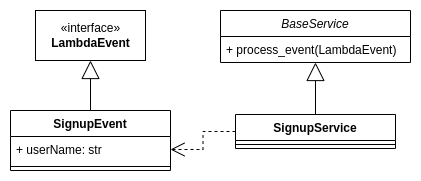
\includegraphics[width=8cm]{sezioni/images/cd_signup.png}
    \centering
    \caption{Signup Service - Diagramma delle classi}
\end{figure}

\subsubsection{Schemi I/O}
\paragraph*{Input}\aCapo{}
Evento \textit{pre signup} in format JSON\G{}, come definito nella documentazione di Cognito\G.

\paragraph*{Output}\aCapo{}
Evento \textit{pre signup} in format JSON\G{} (lo stesso ottenuto in input).
